% !TEX root=../main.tex
\section{Results}
\label{sec:results}

We were pleased to be able to succesffully implement autonomous control of a turtlebot using only visual data. The classical approach served as a meaningful learning experience and also a useful tool in collecting data to train the neural network approach, which was our end goal.

\begin{figure}[hbt]
  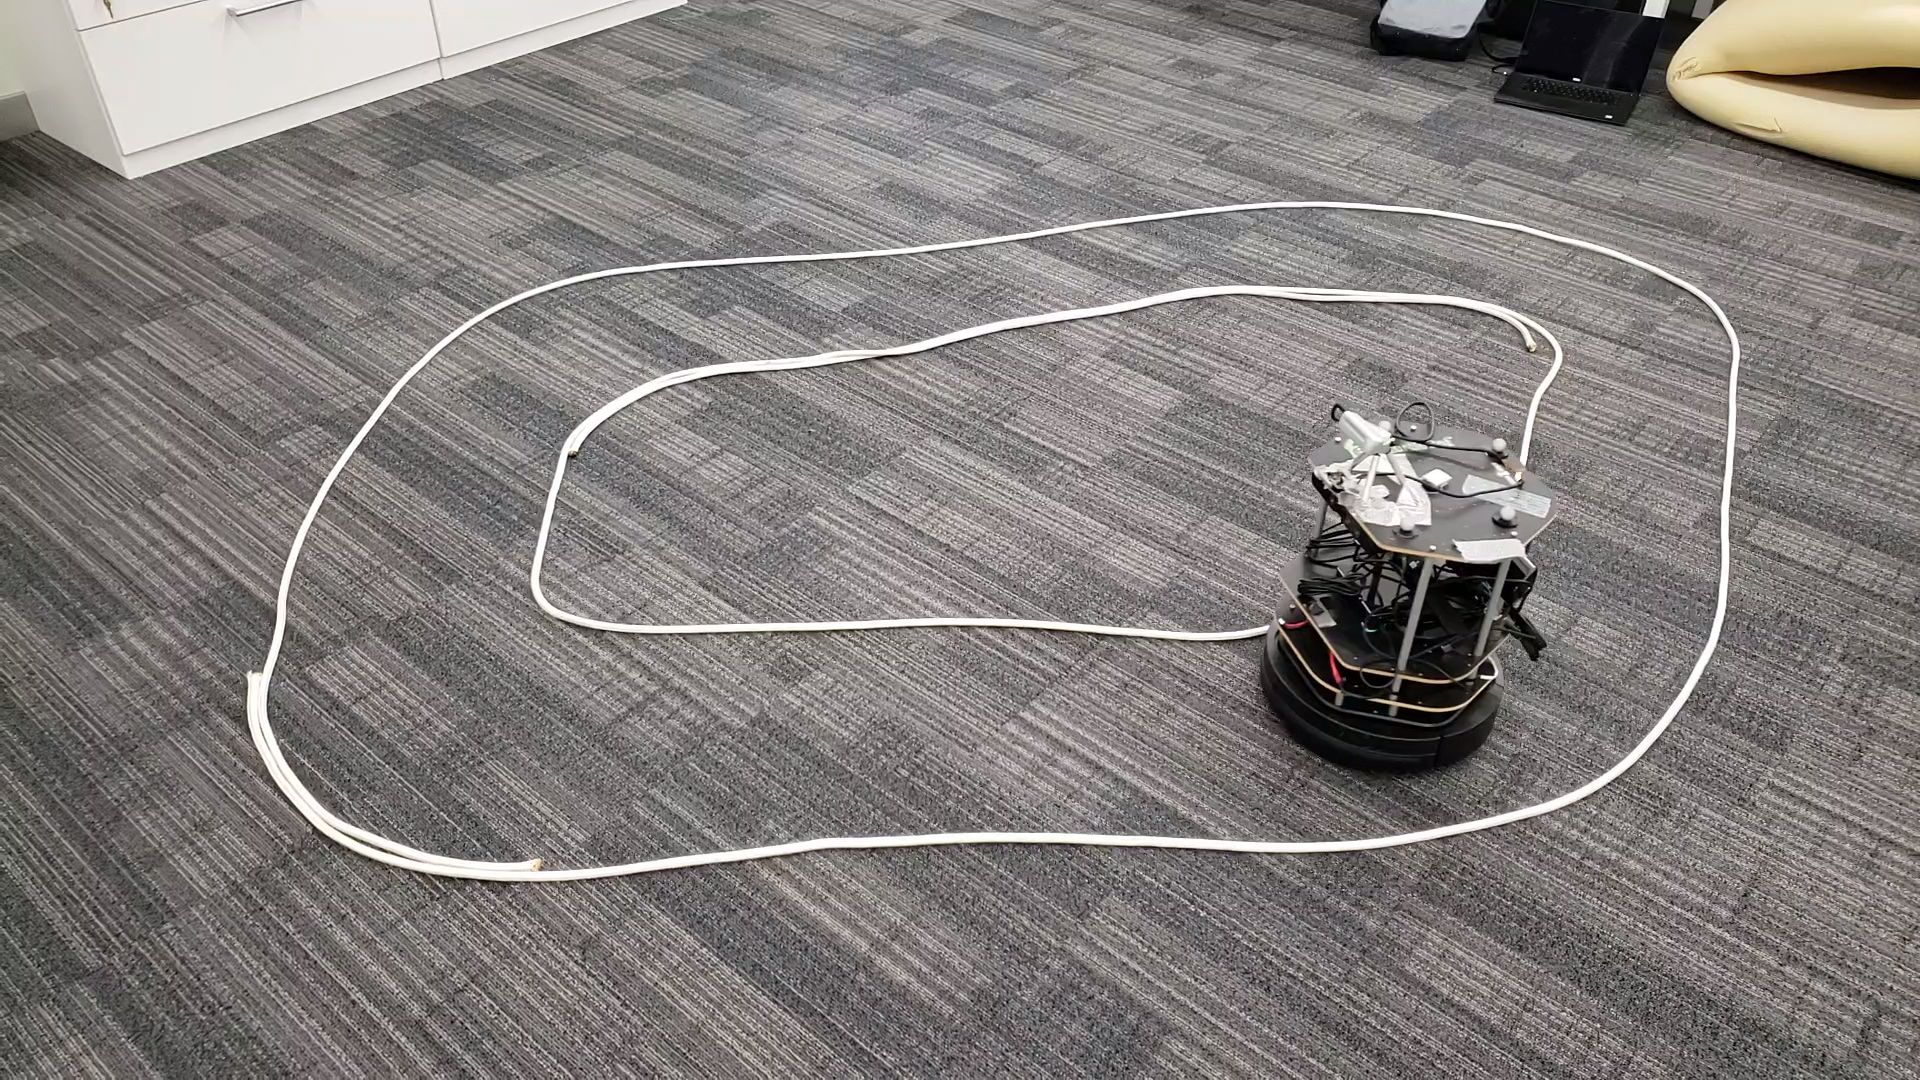
\includegraphics[width=\columnwidth]{figures/success_track}
  \caption{Snapshot of the turtlebot successfully following a track using end-to-end deep learning-based control.}
  \label{fig:success_track}
\end{figure}

Some of the main advantages we saw of using the neural network control as opposed to the classical method was the ability to implicitly encode variability and robustness into the control simply by training on more data in varied environments. For example, the classical method, which depended heavily on proper segmentation, needed to be re-tuned for each ground surface and lighting condition, whereas the neural network was able to learn how to extract the proper features in multiple environments without the need to explicitly retune or revise the network.

It was also interesting to note the information the neural network was able to learn. As a simple metric of determing what the network deemed important, we took the gradient of the output with respect to the input image and, after normalizing the image, were able to visualize which pixels contributed most strongly to the output. As seen in Figures~\ref{fig:saliency1}~through~\ref{fig:saliency3}, the brightest pixels in the gradient image corresponds to the areas where the rope is seen in the input image. Note specifically how the neural network learned to identify the rope specifically, not just white objects, as the light reflection in Figure~\ref{fig:saliency3} is filtered out and does not contribute much to the output. These glare spots were difficult for the classical method to handle, which conveys a clear advantage of the network-based control over the classical control.

\begin{figure}[hbt]
  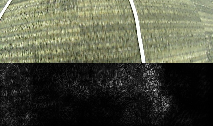
\includegraphics[width=\columnwidth]{figures/saliency1}
  \caption{Top: Original image; bottom: Class saliency for rope on carpet data. Shows the gradient is highest near where the rope appears in the original image (top)}
  \label{fig:saliency1}
\end{figure}

\begin{figure}[hbt]
  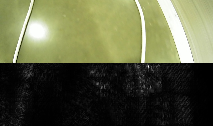
\includegraphics[width=\columnwidth]{figures/saliency2}
  \caption{Class saliency on reflective concrete flooring.}
  \label{fig:saliency2}
\end{figure}

\begin{figure}[hbt]
  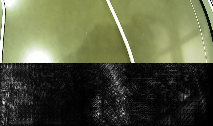
\includegraphics[width=\columnwidth]{figures/saliency3}
  \caption{Class saliency on reflecitve concrete floor with mulptiple glare spots. Show that the network learned to filter out bright contours that do not correspond with rope.}
  \label{fig:saliency3}
\end{figure}
